\documentclass[12pt]{report}

\usepackage[a4paper]{geometry}
%\geometry{left=2.5cm,right=2.5cm,top=2.5cm,bottom=2.5cm, a4paper}
\usepackage[utf8]{inputenc}
\usepackage{amsmath}
\usepackage{amsthm}
\usepackage{amssymb}
\usepackage{ulem}
\usepackage{graphicx}
\usepackage{caption}
\graphicspath{}
\usepackage[document]{ragged2e}
\usepackage{setspace}
\usepackage{tabularx}
\usepackage[slovene]{babel}
\usepackage{textcomp, gensymb}
\usepackage{siunitx}
\usepackage{pdfrender,xcolor}
\usepackage{hyperref}
\usepackage{xurl}
\usepackage{float}
\usepackage{titlesec}

\newfloat{slika}{htbp}{loc}
\floatname{slika}{Slika}

\newfloat{tabela}{htbp}{loc}
\floatname{tabela}{Tabela}

% Differential
\newcommand{\diff}{\mathrm{d}}

\title{
  
\includegraphics[width=0.4\textwidth]{fmf_logo}\\
  {\small Oddelek za fiziko} \\
  {Franck-Hertzov poskus}\\
  {\small Poročilo pri fizikalnem praktikumu IV}\\

}
\date{}
\author{ Kristofer Č. Povšič \\[5 cm]
 \small  Asistent: Jelena Vesić
}


\titleformat{\chapter}[hang]{\Huge\bfseries}{\thechapter{. }}{0pt}{\Huge\bfseries}

\setlength\parindent{0pt}

\begin{document}

\setcounter{page}{2}

\maketitle

\chapter*{Uvod}

S tem poskusom lahko pokažemo diskretnost energijskih nivojev elektronov v atomu. Plinska trioda vsebuje kapljico živega srebra Hg, plinska faza nad njo pa ima pri temperaturi $200^\circ C$ tlak okoli $1kPa$. V cevi pospešujemo elektrone od katode proti anodni mrežici z napetostjo $U_1$ in jih nato lovimo s kolektorsko anodo, ki elektrone dodatno odbija z majhnim potencialom $U_2$. Merimo tok elektronov $I_2$, ki doseže kolektorsko anodo, tj. tok elektronov, ki uspejo premagati zaustavitveni potencial $U_2$ med anodno mrežico in anodnim kolektorjem. 

Ko povečujemo napetost $U_1$, s katero pospešujemo elektrone, doseže kolektorsko anodo vedno več elektronov. A ko kinetične energije elektronov dosežejo $4.9\si{eV}$ - razliko $\Delta E = E_1 - E_0$ med prvima dvema vzbujenima stanjema Hg atoma - postanejo trki neeleastični. Posledično se elektroni upočasnijo in ne dosežejo kolektorske anode. V odvisnosti od $I_2$ vidimo značilen padec. Pri višjih napetostih, npr. $9.8\si{V}$, imajo elektroni že na sredini pospeševalnega pasu kinetično energijo $4.9\si{eV}$. To je dovolj, da jo izgubijo v neelastičnem trku. Od tukaj do anode mrežice spet pridobijo energijo in drugič neelastično trčijo tik ob anodni mrežici. Spet torej opazimo padec v kolektorskem toku $I_2$. 

\chapter*{Naloga}

\begin{itemize}
  \item Opazuj odvisnost toka $I_2$ med anodno mrežico in anodnim kolektorjem v odvisnosti od negativne napetosti $U_1$ na katodi. Spreminjaj temperaturo in posebej natančno opazuj in izmeri položaje vseh vrhov v merjenih odvisnostih. Skiciraj odvisnosti pri petih različnih temperaturah, ko se slike primerno razlikujejo, tj. približno pri temperaturah okoli 180, 160, 140, 120 $^\circ C$ in na koncu še pri sobni temperaturi. 
  \item Natančno določi položaje vrhov $U_{1,n} = U_2 + n\Delta E/e_0$ pri posameznih temperaturah in rezultate vnesi v tabelo. Razlike napetosti med zaporednimi maksimumi ustrezajo energiji, ki jo izgubijo elektroni pri posameznem neelastičnem trku z atomom Hg. Določi $\Delta E = E_1 - E_0 = e_0 \Delta U_1$, kjer sta $E_1$ in $E_0$ energiji prvega vzbujenega in osnovnega stanja elektrona v zunanji lupini Hg. 
\end{itemize}

\begingroup
\let\clearpage\relax

\chapter*{Potrebščine}
\begin{itemize}
  \item Franck-Hertzova cev v termostatiranem ohišju
  \item generator žagaste napetosti in izvor izmenične napetosti za gretje katode ($5.42 \si{V}$. $215\si{mA}$)
  \item digitalni osciloskop (Tektronix serija 2000)
  \item USB ključek za shranjevanje podatkov
\end{itemize}

\chapter*{Navodila in obdelava podatkov }
Prižgem komoro, da se Franck-Hertzova cev začne segrevati. Pri temperaturah 180, 160, 140, 120 in 40 $^\circ C$ pomerim odvisnost $U_2(U_1)$. Pri tem je $U_2$ le napetosti, ki je preko upora $R=1k\Omega$ povezava s kolektorskim tokom $I_2 = U_2 / R $. Iz grafov razberemo relativne višine maksimumov kolektorskega toka $I_2$ in pripadajoče pospeševalne napetosti $U_1$. Iz tega lahko nato izračunamo, da so razmiki med vrhovi: 

\[ \Delta E = (5.0 \pm 0.7) \si{eV}\]
\endgroup

\chapter*{Grafi in tabele}

\begin{slika}[H]
  \centering 
  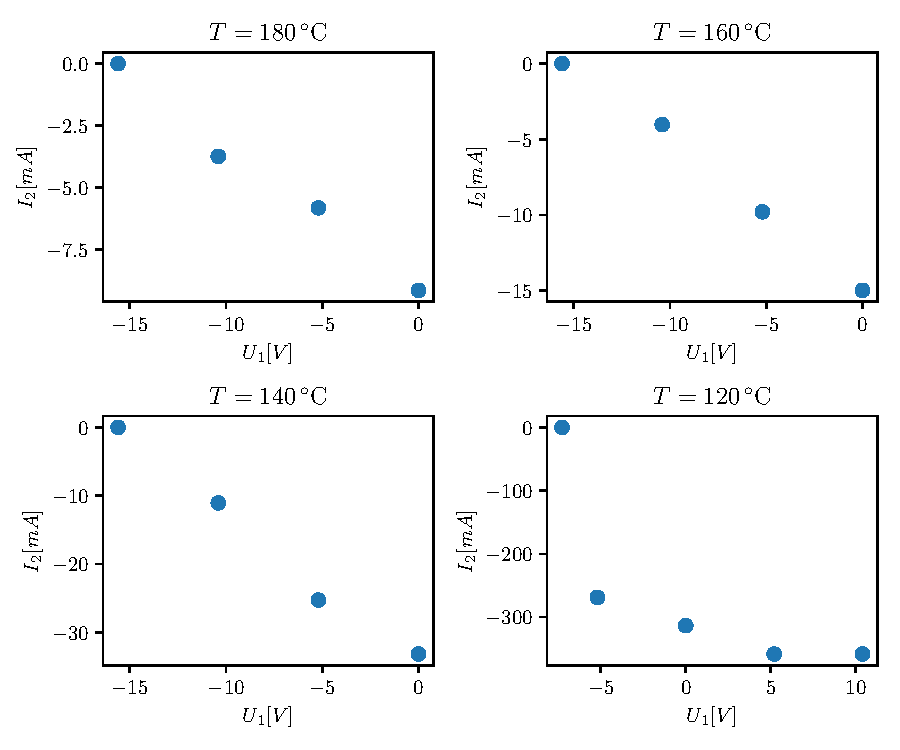
\includegraphics{grafi.pdf}
  \caption{\small Tok v odvisnosti od napetosti na kolektorski katodi. Odvisnost je izmerjena pri temperaturah 180, 160, 140, 120 $^\circ C$}
\end{slika}

\begin{slika}[H]
  \centering
  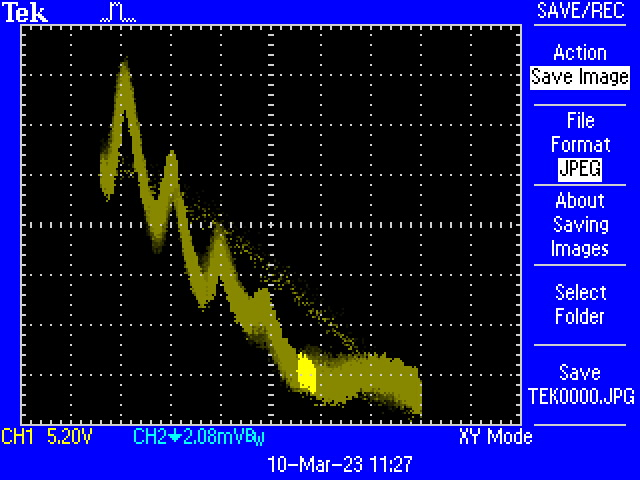
\includegraphics[width= 0.75\textwidth]{TEK0000}
  \caption{\small Graf osciloskopa pri temperaturi 180 $^\circ C$}
\end{slika}

\begin{tabela}[H]
  \centering
  \[
      \begin{array}{|c|c|c|} \hline
        U_1 [\si{V}] & U_2 [\si{mV}] \\ \hline
        -15.60 &    6.24\\
        -10.40 &    2.50\\
         -5.20 &    0.42\\
          0.00 &  -2.91 \\ \hline
    \end{array}
  \]
  \caption{\small Tabela vrednosti iz osciloskopa pri temperaturi 180 $^\circ C$}
\end{tabela}

\begin{slika}[H]
  \centering
  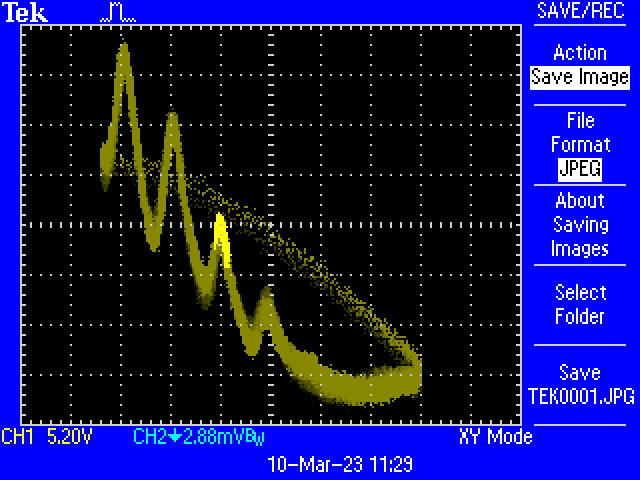
\includegraphics[width= 0.75\textwidth]{TEK0001}
  \caption{\small Graf osciloskopa pri temperaturi 160 $^\circ C$}
\end{slika}

\begin{tabela}[H]
  \centering
  \[
      \begin{array}{|c|c|c|} \hline
        U_1 [\si{V}] & U_2 [\si{mV}] \\ \hline
        -15.60 &   10.37\\
        -10.40 &    6.34\\
         -5.20 &    0.58\\
           0.00 &  -4.61 \\ \hline
    \end{array}
  \]
  \caption{\small Tabela vrednosti iz osciloskopa pri temperaturi 160 $^\circ C$}
\end{tabela}

\begin{slika}[H]
  \centering
  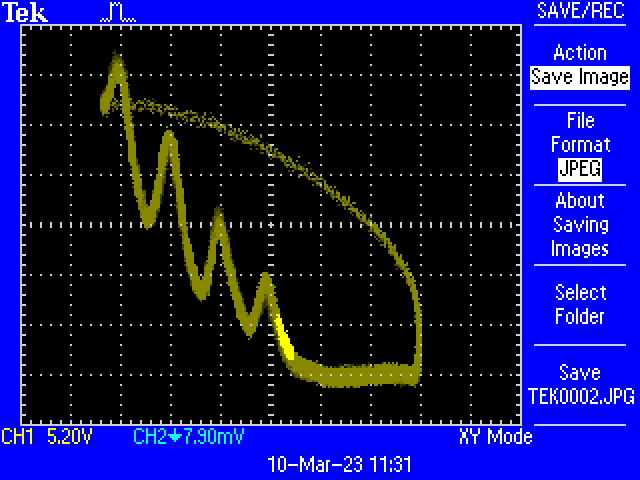
\includegraphics[width= 0.75\textwidth]{TEK0002}
  \caption{\small Graf osciloskopa pri temperaturi 140 $^\circ C$}
\end{slika}

\begin{tabela}[H]
  \centering
  \[
      \begin{array}{|c|c|c|} \hline
        U_1 [\si{V}] & U_2 [\si{mV}] \\ \hline
        -15.60 &   25.28\\
        -10.40 &   14.22\\
         -5.20 &    0.00\\
           0.00 &  -7.90 \\ \hline
    \end{array}
  \]
  \caption{\small Tabela vrednosti iz osciloskopa pri temperaturi 140 $^\circ C$}
\end{tabela}

\begin{slika}[H]
  \centering
  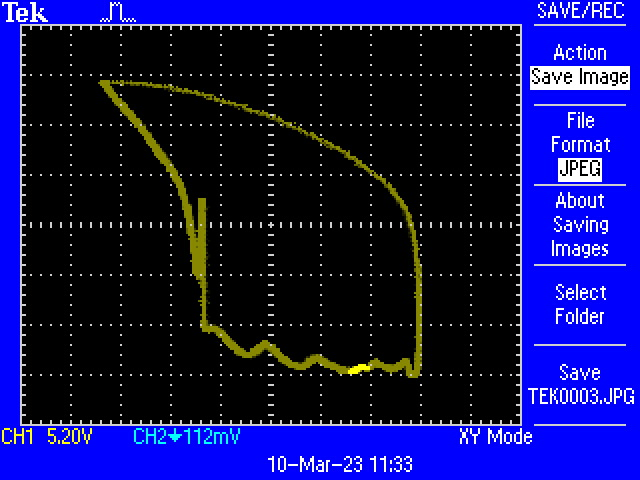
\includegraphics[width= 0.75\textwidth]{TEK0003}
  \caption{\small Graf osciloskopa pri temperaturi 120 $^\circ C$}
\end{slika}

\begin{tabela}[H]
  \centering
  \[
      \begin{array}{|c|c|c|} \hline
        U_1 [\si{V}] & U_2 [\si{mV}] \\ \hline
        -7.28 &   44.80\\
        -5.20 & -224.00\\
          0.00 & -268.80\\
          5.20 & -313.60\\
         10.40 & -313.60 \\ \hline
    \end{array}
  \]
  \caption{\small Tabela vrednosti iz osciloskopa pri temperaturi 120 $^\circ C$}
\end{tabela}

\begin{slika}[H]
  \centering
  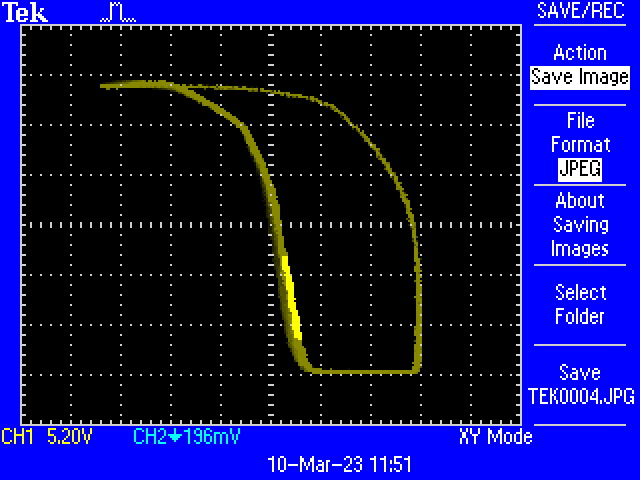
\includegraphics[width= 0.75\textwidth]{TEK0004}
  \caption{\small Graf osciloskopa pri temperaturi 40 $^\circ C$}
\end{slika}



\end{document}